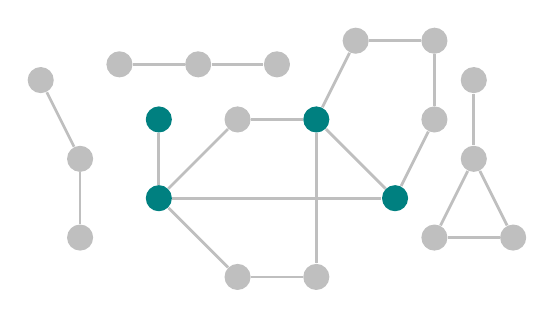
\begin{tikzpicture}
\tikzstyle{node_style1} = [circle,fill=teal]
\tikzstyle{node_style2} = [circle,fill=lightgray]
\tikzstyle{edge_style1} = [black, line width=1]
\tikzstyle{edge_style2} = [lightgray, line width=1]
    \node[node_style1] (v1) at (0,1) {};
    \node[node_style2] (v2) at (1,2) {};
    \node[node_style1] (v3) at (2,2) {};
    \node[node_style2] (v4) at (2.5,3) {};
    \node[node_style2] (v5) at (3.5,3) {};
    \node[node_style2] (v6) at (3.5,2) {};
    \node[node_style1] (v7) at (3,1) {};
    \node[node_style2] (v8) at (2,0) {};
    \node[node_style2] (v9) at (1,0) {};
    \node[node_style1] (v10) at (0,2) {};

    \draw[edge_style2] (v1) edge (v2);
    \draw[edge_style2] (v1) edge (v7);
    \draw[edge_style2] (v1) edge (v9);
    \draw[edge_style2] (v1) edge (v10);
    \draw[edge_style2] (v2) edge (v3);
    \draw[edge_style2] (v3) edge (v4);
    \draw[edge_style2] (v3) edge (v7);
    \draw[edge_style2] (v3) edge (v8);
    \draw[edge_style2] (v4) edge (v5);
    \draw[edge_style2] (v5) edge (v6);
    \draw[edge_style2] (v6) edge (v7);
    \draw[edge_style2] (v8) edge (v9);

    \node[node_style2] (v21) at (-1,0.5) {};
    \node[node_style2] (v22) at (-1,1.5) {};
    \node[node_style2] (v23) at (-1.5,2.5) {};
                                                
    \draw[edge_style2] (v21) edge (v22);
    \draw[edge_style2] (v22) edge (v23);

    \node[node_style2] (v31) at (-0.5, 2.7) {};
    \node[node_style2] (v32) at (0.5,2.7) {};
    \node[node_style2] (v33) at (1.5,2.7) {};

    \draw[edge_style2] (v31) edge (v32);
    \draw[edge_style2] (v32) edge (v33);

    \node[node_style2] (v41) at (3.5, 0.5) {};
    \node[node_style2] (v42) at (4.5, 0.5) {};
    \node[node_style2] (v43) at (4, 1.5) {};
    \node[node_style2] (v44) at (4, 2.5) {};
                                                
    \draw[edge_style2] (v41) edge (v42);
    \draw[edge_style2] (v41) edge (v43);
    \draw[edge_style2] (v42) edge (v43);
    \draw[edge_style2] (v43) edge (v44);
\end{tikzpicture}
